\documentclass[11pt,a4paper]{article}
\usepackage[margin=2.1cm,top=2cm,bottom=2cm]{geometry}
% Préambule commun aux deux documents
\usepackage[T1]{fontenc}
\usepackage[french]{babel}
\usepackage{lmodern}
\usepackage{amsmath,amssymb}
\usepackage{graphicx,xcolor,booktabs,array,tabularx,longtable}
\usepackage{tikz}
\usetikzlibrary{positioning,arrows.meta,shapes.geometric,calc,fit,backgrounds,decorations.pathreplacing}
\usepackage{fancyhdr,enumitem,microtype}
\usepackage[colorlinks=true,linkcolor=aegis,urlcolor=aegis,citecolor=aegis]{hyperref}
\usepackage{caption}
\usepackage{listings}

\definecolor{aegis}{RGB}{14,116,144}
\definecolor{aegisfonce}{RGB}{11,18,32}
\definecolor{grisfond}{RGB}{247,248,250}
\definecolor{grisligne}{RGB}{216,220,226}
\definecolor{gristexte}{RGB}{91,97,107}
\definecolor{vertok}{RGB}{26,127,75}
\definecolor{orangepartiel}{RGB}{178,106,5}
\definecolor{rougeko}{RGB}{198,40,40}

\captionsetup{font=small,labelfont={bf,color=aegis}}
\setlist[itemize]{leftmargin=1.2em,itemsep=1pt,topsep=2pt,parsep=0pt}
\setlist[enumerate]{leftmargin=1.4em,itemsep=1pt,topsep=2pt,parsep=0pt}

\lstset{
  basicstyle=\ttfamily\scriptsize,
  backgroundcolor=\color{grisfond},
  frame=single, rulecolor=\color{grisligne},
  breaklines=true, showstringspaces=false,
  keywordstyle=\color{aegis}\bfseries,
  commentstyle=\color{gristexte}\itshape,
  numberstyle=\tiny\color{gristexte},
  xleftmargin=4pt, framexleftmargin=4pt, aboveskip=6pt, belowskip=6pt,
  literate={é}{{\'e}}1 {è}{{\`e}}1 {à}{{\`a}}1 {ç}{{\c c}}1 {ê}{{\^e}}1 {û}{{\^u}}1 {î}{{\^i}}1 {ô}{{\^o}}1 {É}{{\'E}}1 {—}{{---}}1 {’}{{'}}1 {«}{{<<}}1 {»}{{>>}}1 {·}{{\textperiodcentered}}1
}

% Marqueurs d'état
\newcommand{\ok}{\textcolor{vertok}{\textbf{Atteint}}}
\newcommand{\partiel}{\textcolor{orangepartiel}{\textbf{Partiel}}}
\newcommand{\absent}{\textcolor{rougeko}{\textbf{Non traité}}}
\newcommand{\plus}{\textcolor{aegis}{\textbf{Au-delà}}}

% Mesure mise en avant dans le fil du texte
\newcommand{\mesure}[1]{\textcolor{aegis}{\textbf{#1}}}

% Les paragraphes techniques enchaînent de longues suites en \texttt{} que TeX
% ne peut pas couper : sans marge de man\oe{}uvre, elles débordent dans la marge.
\emergencystretch=2em
\hbadness=4000

\usepackage{lastpage}
\pagestyle{fancy}\fancyhf{}
\renewcommand{\headrulewidth}{0.4pt}
\fancyhead[L]{\small\textcolor{gristexte}{Dossier technique --- AEGIS Mini-SOC}}
\fancyhead[R]{\small\textcolor{gristexte}{v1.0.0}}
\fancyfoot[C]{\small\thepage\ / \pageref{LastPage}}
\setlength{\parskip}{3pt}\setlength{\parindent}{0pt}

\begin{document}

\begin{center}
{\LARGE\bfseries Dossier technique --- AEGIS Mini-SOC}\\[3pt]
{\large Spécification complète, protocole de mesure et résultats détaillés}\\[6pt]
{\small Mohamed Aziz BAOUEB \quad\textbullet\quad \url{https://github.com/aziz3r/aegis-mini-soc}}
\end{center}
\rule{\linewidth}{0.8pt}

\small
\textit{Ce document accompagne le rapport de projet. Il rassemble la spécification exhaustive du
système --- caractéristiques, modèles, API, modèle de données, inventaire des tests --- ainsi que
les résultats complets, famille par famille, et le détail du protocole qui les produit.}
\normalsize

\tableofcontents
\clearpage

%================================================================================
\part*{Partie I --- Spécification du système}
\addcontentsline{toc}{section}{Partie I --- Spécification du système}

\section{Vue générale}

\subsection{Nature et périmètre}

AEGIS est un système de détection d'intrusion réseau (NIDS) \textbf{comportemental}, accompagné
d'une interface de supervision et de triage. Il n'utilise aucune base de signatures : il apprend la
distribution du trafic normal et signale les écarts.

\begin{table}[h]\centering\small
\begin{tabularx}{\linewidth}{@{}l X@{}}
\toprule
Nature & Détection d'intrusion réseau comportementale + poste d'analyste \\
Langages & Python 3.11+ (moteur, API) ; TypeScript 5 strict (interface) \\
Volume & $\approx$9\,800 lignes : 5\,800 backend, 3\,100 interface, 900 tests \\
Tests & 94, tous passants \\
Déploiement & mono-processus, sans dépendance système ; PostgreSQL optionnel \\
Démarrage & \texttt{./scripts/demo.sh} \\
Licence & MIT \\
\bottomrule
\end{tabularx}
\end{table}

\subsection{Chaîne de traitement}

\begin{figure}[h]\centering
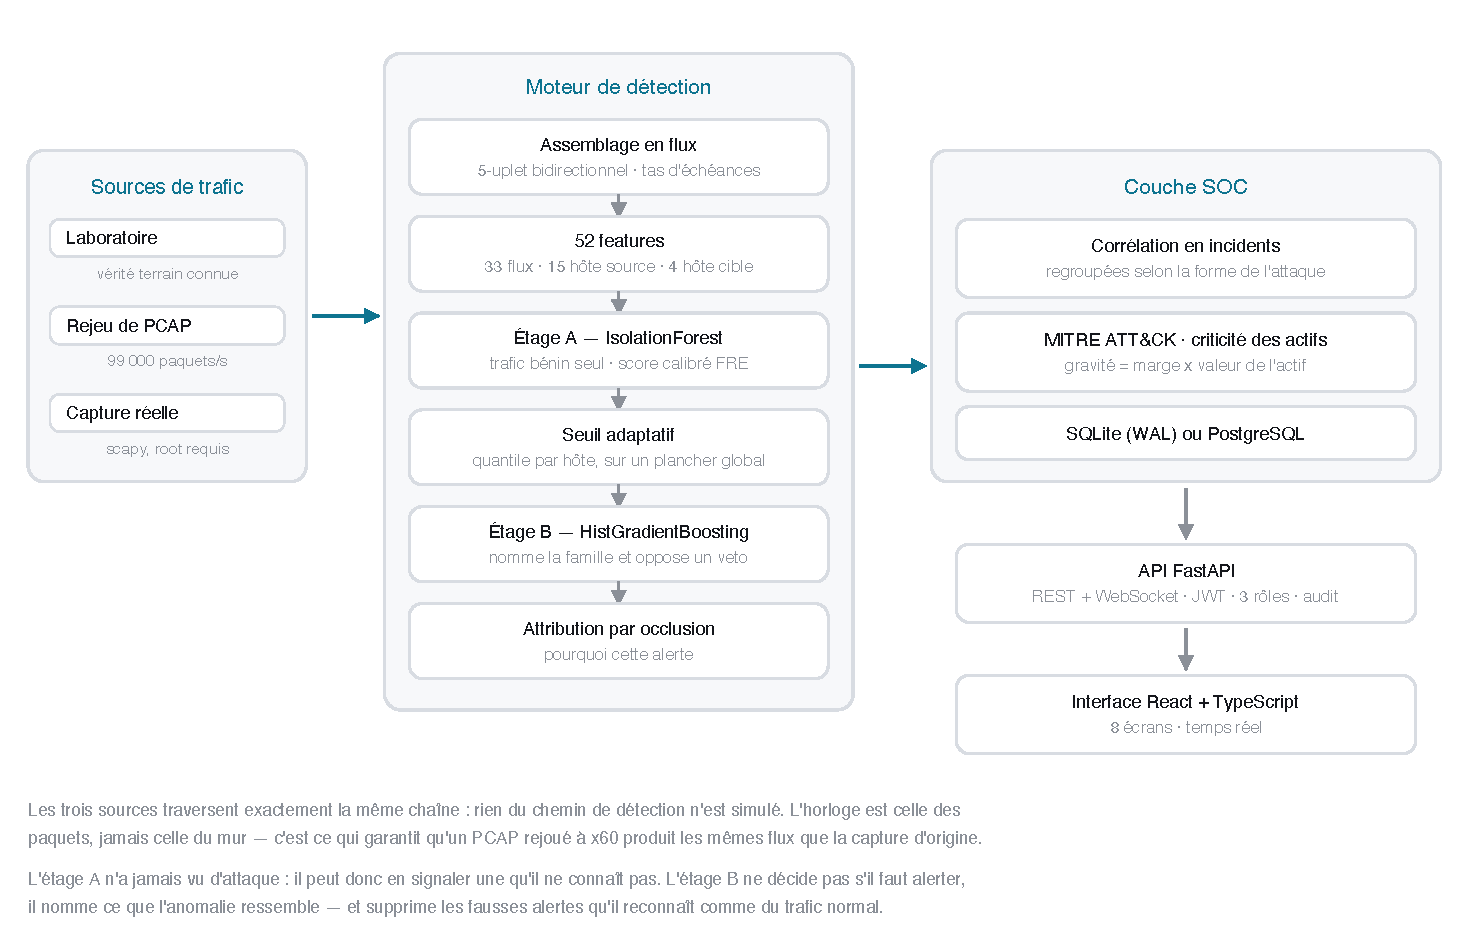
\includegraphics[width=\linewidth]{../docs/architecture.pdf}
\caption{La chaîne complète, des paquets jusqu'à l'interface.}
\end{figure}

Trois sources de trafic alimentent indifféremment le même moteur : un réseau de laboratoire
synthétique produisant des paquets étiquetés, un fichier PCAP rejoué, ou une interface réseau
réelle. Le reste de la chaîne ignore la provenance.

%================================================================================
\section{Assemblage en flux}

\subsection{Définition de l'unité d'analyse}

L'unité analysée est le \textbf{flux bidirectionnel}, identifié par son 5-uplet canonique
(adresse source, adresse destination, port source, port destination, protocole), rendu
indépendant du sens de manière à ce que \texttt{A$\rightarrow$B} et \texttt{B$\rightarrow$A}
constituent un seul flux.

\subsection{Déclencheurs d'export}

\begin{table}[h]\centering\small
\begin{tabularx}{\linewidth}{@{}l l X@{}}
\toprule
\textbf{Déclencheur} & \textbf{Délai} & \textbf{Justification} \\
\midrule
Fin de connexion TCP & immédiat & RST observé, ou FIN dans les deux sens \\
Connexion sans réponse & 3 s & un SYN sans réponse est déjà une observation complète \\
Inactivité & 15 s & plus aucun paquet n'est observé sur le flux \\
Durée d'ouverture & 120 s & un flux long est exporté par tranches, pour rester visible \\
\bottomrule
\end{tabularx}
\end{table}

\begin{figure}[h]\centering
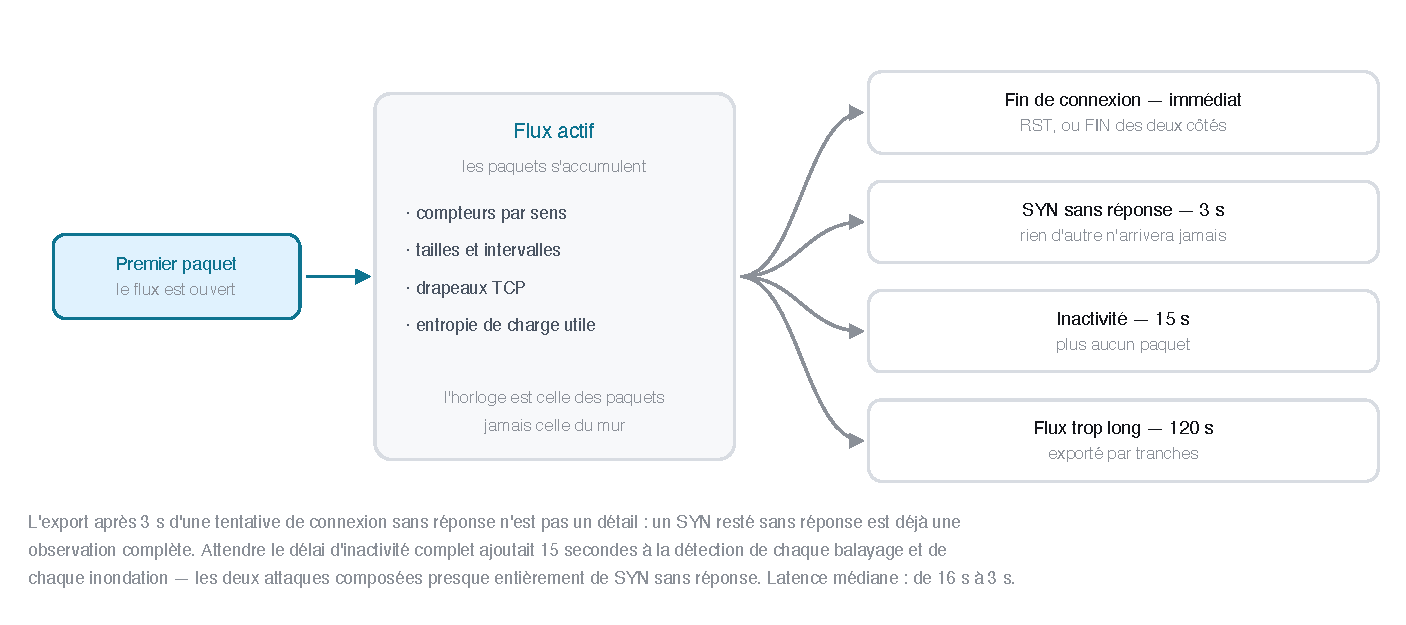
\includegraphics[width=0.94\linewidth]{../docs/cycle-de-vie.pdf}
\caption{Les quatre façons dont un flux quitte la table.}
\end{figure}

Le cas des connexions sans réponse n'est pas un détail d'optimisation. Un balayage de ports et une
inondation SYN sont composés presque entièrement de tentatives sans réponse ; les conserver pendant
le délai d'inactivité complet ajoutait quinze secondes à leur détection. Le délai dédié de trois
secondes a ramené la latence médiane de détection de seize à trois secondes.

\subsection{Mécanique d'expiration}

L'expiration repose sur deux tas d'échéances paresseux : un pour l'inactivité, un pour la durée
d'ouverture. Chaque paquet empile une échéance ; les entrées périmées --- le flux a reçu un paquet
depuis, ou a déjà été exporté --- sont reconnues au dépilage grâce à un compteur de génération
propre à chaque flux, puis rejetées.

\begin{table}[h]\centering\small
\begin{tabularx}{\linewidth}{@{}X r r@{}}
\toprule
\textbf{Implémentation} & \textbf{Complexité par paquet} & \textbf{Débit mesuré} \\
\midrule
Parcours de la table des flux actifs & $O(n_{\text{actifs}})$ & 12\,000 paquets/s \\
Tas d'échéances paresseux & $O(\log n)$ amorti & \mesure{33\,000 paquets/s} \\
\bottomrule
\end{tabularx}
\end{table}

L'équivalence stricte entre les deux implémentations est vérifiée par un test, sur quatre minutes de
trafic mixte : les flux produits sont identiques en identité, nombre de paquets et volume. Une
optimisation non prouvée est un bug qui attend.

\subsection{Horloge}

Le champ \texttt{Packet.ts} porte toujours l'horloge de \textbf{capture}, jamais l'heure d'arrivée
réelle. Les délais d'expiration s'expriment donc en temps de capture, ce qui garantit qu'un fichier
PCAP rejoué à soixante fois la vitesse produit exactement les mêmes flux que la capture d'origine.
L'heure d'arrivée est enregistrée séparément, pour l'affichage uniquement.

%================================================================================
\section{Les 52 caractéristiques}

\subsection{Caractéristiques intrinsèques au flux (33)}

\begin{table}[h]\centering\small
\begin{tabularx}{\linewidth}{@{}l X@{}}
\toprule
\textbf{Sous-groupe} & \textbf{Caractéristiques} \\
\midrule
Volume & durée, paquets aller, paquets retour, paquets totaux, octets aller, octets retour,
octets totaux \\
Débit & paquets par seconde, octets par seconde \\
Dissymétrie & ratio paquets aller/retour, ratio octets descendant/montant \\
Tailles & moyenne, écart-type, minimum, maximum \\
Temporalité & intervalle moyen, écart-type, minimum, maximum \\
Drapeaux TCP & SYN, ACK, FIN, RST, PSH, URG, poignée de main aboutie \\
Protocole & TCP, UDP, ICMP (trois indicatrices) \\
Charge utile & longueur moyenne, entropie de Shannon normalisée, part de paquets sans données \\
Port & le port de destination est-il un port système ($<1024$) \\
\bottomrule
\end{tabularx}
\end{table}

\subsection{Comportement de l'hôte source (15)}

Mesuré sur deux fenêtres glissantes, dix et soixante secondes : nombre de flux, destinations
distinctes, ports distincts, taux de SYN sans établissement, part de connexions échouées, octets
sortants et entrants, ratio sortant/entrant, part de destinations jamais contactées auparavant,
durée moyenne des flux, répétitions maximales vers une même cible, et \textbf{régularité de type
balise}.

Cette dernière mérite une définition : elle vaut $1 - \mathrm{CV}$, où $\mathrm{CV}$ est le
coefficient de variation des intervalles entre contacts successifs vers la destination la plus
sollicitée. Une valeur proche de 1 traduit une périodicité d'horloge --- ce que fait un implant qui
contacte son serveur de commande, et ce qu'un humain ne fait jamais.

\subsection{Comportement de l'hôte destination (4)}

Nombre de flux reçus, sources distinctes, taux de SYN non établis et part de connexions échouées,
sur dix secondes.

Ces quatre caractéristiques existent pour un cas précis : une inondation dont les adresses sources
sont \textbf{usurpées} est invisible côté source, puisque chaque adresse falsifiée n'émet qu'un seul
paquet et paraît donc inactive. Seule l'agrégation sur la victime la rend détectable.

\subsection{Une absence volontaire}

Le numéro de port de destination \emph{brut} n'est pas une caractéristique. Un modèle à arbres le
mémoriserait --- 22 pour la force brute SSH, 53 pour le tunnel DNS --- et afficherait des scores
excellents sans aucun rapport avec sa capacité à généraliser sur du trafic réel. Seules les
propriétés structurelles du port sont conservées.

\subsection{Garantie d'ordre}

La liste \texttt{FEATURE\_NAMES} est l'unique source de vérité pour l'ordre des colonnes. Le modèle
enregistre cette liste et \textbf{refuse de se charger} si elle a changé : une colonne qui se
décale silencieusement est le pire mode de panne d'un système de ce type, puisqu'il continue de
produire des scores d'apparence normale.

%================================================================================
\section{Le modèle à deux étages}

\subsection{Étage A --- détection d'anomalie non supervisée}

\begin{table}[h]\centering\small
\begin{tabularx}{\linewidth}{@{}l X@{}}
\toprule
Algorithme & IsolationForest, 220 arbres, \texttt{max\_samples}~=~4096 \\
Normalisation & RobustScaler, quantiles 5--95 \\
Contamination & 0,02 --- une capture \og{}bénigne\fg{} contient toujours un peu d'étrangeté réelle \\
Entraînement & \textbf{trafic bénin exclusivement}, 22\,295 flux \\
Sortie brute & score non borné, non interprétable \\
\bottomrule
\end{tabularx}
\end{table}

N'ayant jamais vu d'attaque, cet étage peut en signaler une qu'il ne connaît pas. C'est la propriété
qui justifie l'approche comportementale, et elle serait perdue si on l'entraînait sur des attaques
étiquetées.

\subsection{Calibration par fonction de répartition empirique}

La sortie brute d'un IsolationForest n'est pas interprétable : elle dépend de l'échelle des données
et n'a pas d'unité. Elle est donc passée par la fonction de répartition empirique des scores obtenus
sur le \textbf{trafic bénin d'entraînement}.

Le score devient alors un percentile : 0,97 signifie \og{}plus inhabituel que 97\% du trafic normal
connu\fg{}. Un seuil posé sur ce nombre est directement lisible comme un budget de faux positifs.

Au-delà du maximum observé en trafic bénin, la fonction ne sature pas : elle tend vers 1 de façon
asymptotique, ce qui préserve l'ordre entre deux anomalies toutes deux extrêmes.

\textbf{Validation :} appliquée à une loi normale, la calibration retrouve la fonction de répartition
de cette loi à $\pm$0,01 près (0 $\rightarrow$ 0,500 ; 1 $\rightarrow$ 0,841 ; 1,96 $\rightarrow$
0,975). C'est un test de la suite.

\subsection{Étage B --- classification de la famille}

\begin{table}[h]\centering\small
\begin{tabularx}{\linewidth}{@{}l X@{}}
\toprule
Algorithme & HistGradientBoosting, 300 itérations, 31 feuilles, $L_2 = 1{,}0$ \\
Équilibrage & \texttt{class\_weight="balanced"}, arrêt anticipé sur 15\% de validation \\
Entraînement & 19\,397 flux étiquetés, plafonnés à 2\,500 par classe \\
Sortie & famille et confiance ; \og{}inconnu\fg{} en dessous de 0,55 de confiance \\
\bottomrule
\end{tabularx}
\end{table}

Le plafonnement par classe n'est pas cosmétique : une seule inondation produit des milliers de flux
quasi identiques et représenterait 70\% du jeu d'entraînement, rendant invisibles les familles rares
--- balise, exfiltration --- qui sont précisément les plus difficiles.

Cet étage ne décide pas s'il faut alerter. Il nomme, et refuse de nommer en dessous du seuil de
confiance : une étiquette fausse mais assurée nuit davantage à un analyste qu'une absence
d'étiquette.

\subsection{La cascade de précision}

\begin{figure}[h]\centering
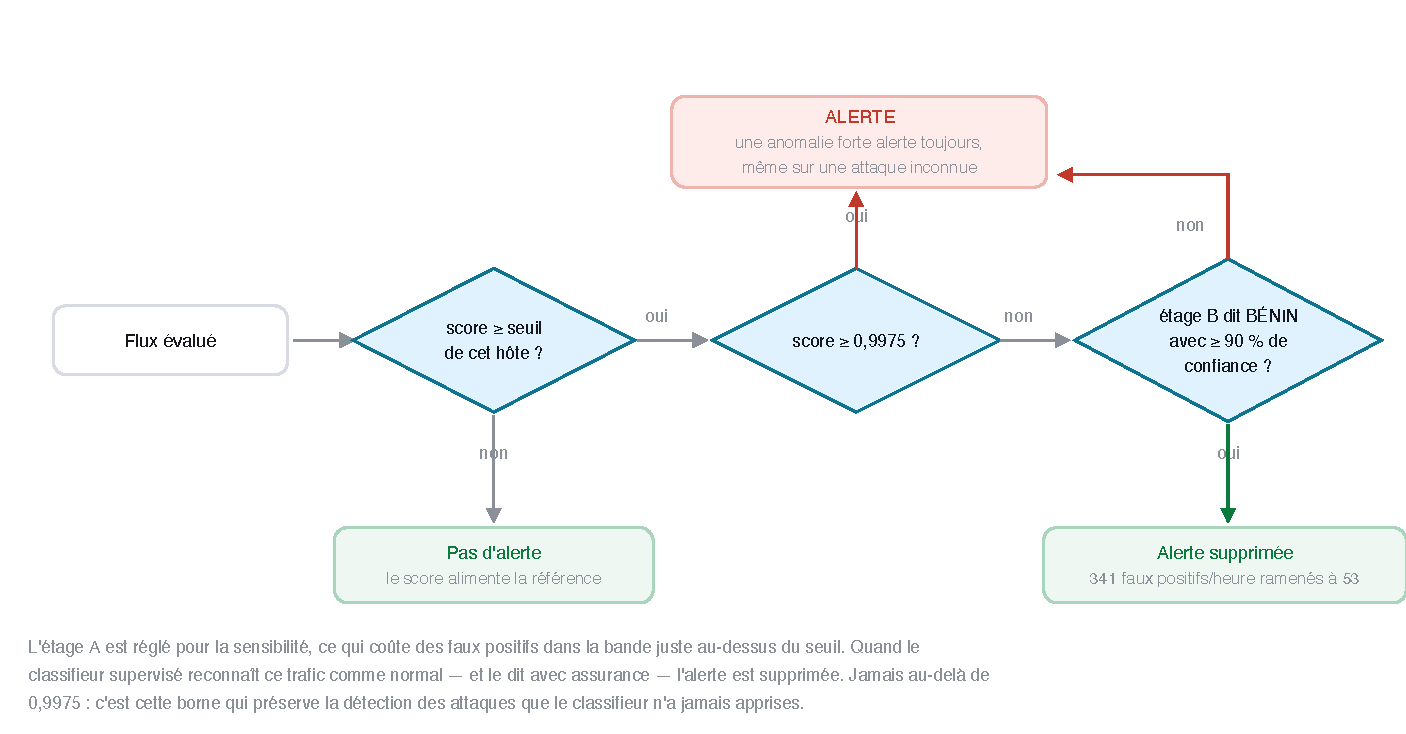
\includegraphics[width=0.92\linewidth]{../docs/cascade.pdf}
\caption{La décision d'alerter, étage par étage.}
\end{figure}

\begin{lstlisting}
seuil      = seuils.threshold(hote)          # lu AVANT apprentissage
alerte     = score >= seuil
si alerte et famille == BENIGN et confiance >= 0.90 et score < 0.9975 :
    alerte = False                           # veto de l'etage B
seuils.observe(hote, score, alerte)          # les alertes n'alimentent pas la reference
\end{lstlisting}

La borne de 0,9975 est ce qui rend la cascade acceptable : au-delà, une anomalie forte alerte
toujours, quoi qu'en dise le classifieur. Sans elle, une attaque jamais apprise serait étouffée par
un modèle qui ne la connaît pas.

\begin{table}[h]\centering\small
\begin{tabularx}{\linewidth}{@{}X r r r@{}}
\toprule
 & \textbf{Faux positifs/h} & \textbf{Rappel bruyant} & \textbf{Rappel furtif} \\
\midrule
Sans cascade & 341 & 99,83\% & 98,78\% \\
Avec cascade & \mesure{53} & 99,82\% & 98,15\% \\
\bottomrule
\end{tabularx}
\caption{Effet mesuré de la cascade : six fois moins de faux positifs pour 0,6 point de rappel furtif.}
\end{table}

\subsection{Attribution par occlusion}

Chaque caractéristique est remplacée tour à tour par sa valeur médiane sur le trafic normal, et le
flux est réévalué ; la chute du score mesure la part de l'anomalie qui lui est imputable. C'est
l'intuition que SHAP formalise, calculée \emph{exactement} pour les sous-ensembles à une
caractéristique, en un seul appel vectorisé et sans dépendance supplémentaire.

Le coût est encadré par un budget : une inondation peut lever des centaines d'alertes par seconde, et
les expliquer toutes dominerait la boucle sans aucun bénéfice, puisqu'elles sont fusionnées en un
seul incident qui n'a besoin que d'une explication. L'incident conserve celle de son alerte la plus
forte.

%================================================================================
\section{Le seuil adaptatif}

\begin{figure}[h]\centering
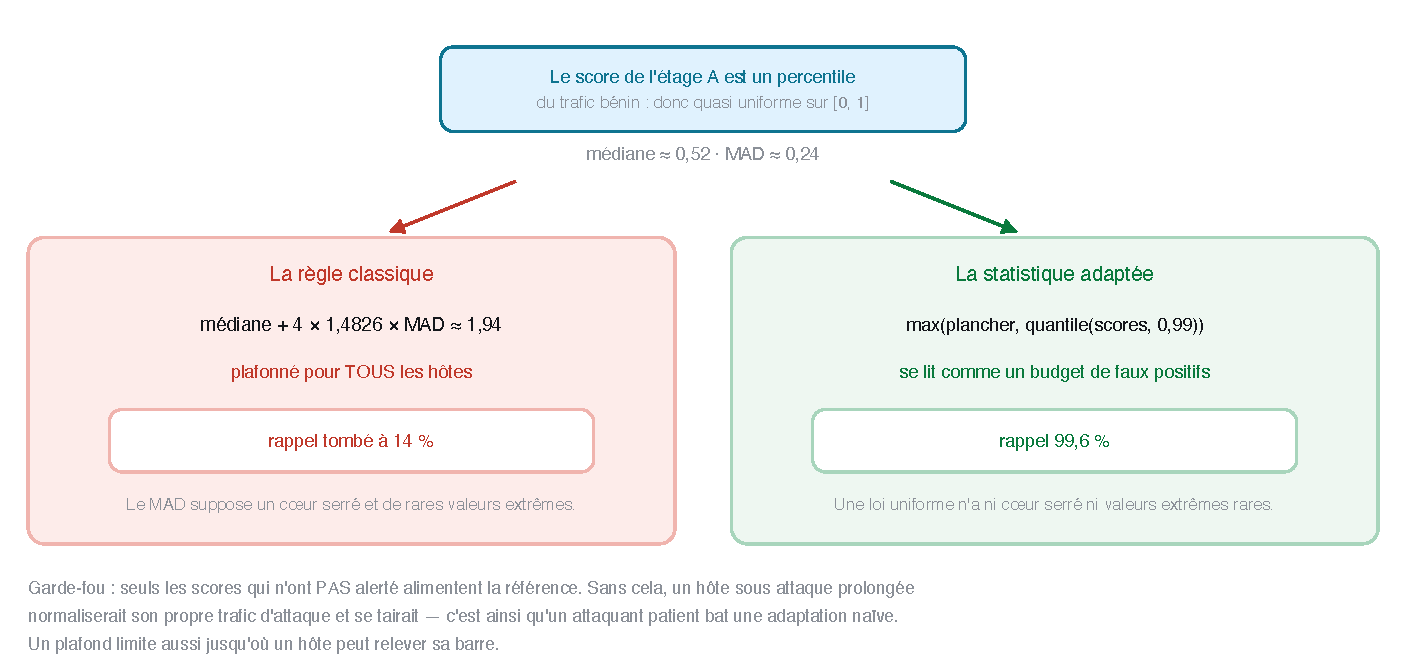
\includegraphics[width=0.92\linewidth]{../docs/seuil.pdf}
\caption{Pourquoi un quantile et non la règle robuste classique.}
\end{figure}

\[
\text{seuil(hôte)} = \mathrm{borner}\Big(\max\big(\text{plancher global},\;
Q_{0,99}(\text{scores de l'hôte})\big)\Big)
\]

\begin{table}[h]\centering\small
\begin{tabularx}{\linewidth}{@{}l r X@{}}
\toprule
\textbf{Paramètre} & \textbf{Valeur} & \textbf{Signification} \\
\midrule
Plancher global & 0,98 & budget de faux positifs, et valeur à froid \\
Quantile par hôte & 0,99 & alerter sur le 1\% le plus inhabituel de cet hôte \\
Plafond & 0,995 & limite jusqu'où un hôte peut relever sa propre barre \\
Référence minimale & 60 flux & en deçà, le plancher s'applique \\
Fenêtre & 512 scores & historique glissant par hôte \\
\bottomrule
\end{tabularx}
\end{table}

\subsection{Pourquoi la règle « médiane + k·MAD » échoue ici}

La première implémentation utilisait cette règle robuste classique. Mesurée, elle a fait tomber le
rappel à \mesure{14\%} --- sans qu'aucune métrique de classement ne le signale, puisque le PR-AUC
restait à 0,993.

La cause : les scores de l'étage A étant déjà des percentiles, ils sont quasi uniformes sur le
trafic normal. La médiane vaut environ 0,52, l'écart absolu médian 0,24, et
$0{,}52 + 4 \times 1{,}4826 \times 0{,}24 \approx 1{,}94$, valeur plafonnée pour \emph{tous} les
hôtes. L'écart absolu médian suppose une distribution à c\oe{}ur serré avec de rares valeurs
extrêmes ; une loi uniforme ne présente ni l'un ni l'autre.

\subsection{Les deux garde-fous}

\textbf{Exclusion des scores alertants.} Seuls les scores n'ayant pas déclenché d'alerte alimentent
la référence. Sans cette règle, un hôte sous attaque prolongée normaliserait progressivement son
propre trafic d'attaque et cesserait d'alerter --- le mode de défaillance dit \og{}de la grenouille
ébouillantée\fg{}, et la manière dont un attaquant patient défait une adaptation naïve. Un test
vérifie que cinq mille scores alertants consécutifs ne déplacent pas le seuil d'un hôte.

\textbf{Plafond.} Un hôte ne peut relever sa barre au-delà de 0,995, afin qu'une attaque lente qui
parviendrait malgré tout à s'infiltrer dans une référence ne puisse pas rendre cet hôte insensible.

%================================================================================
\section{Corrélation et triage}

\begin{figure}[h]\centering
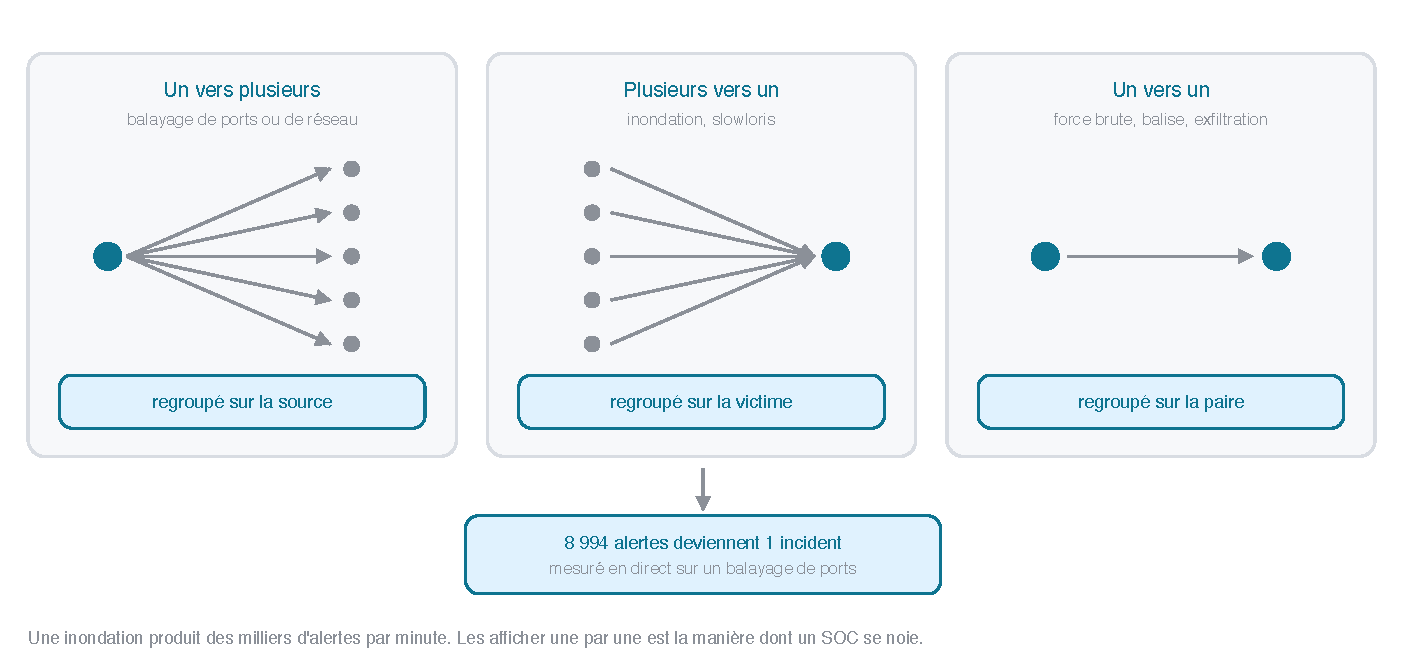
\includegraphics[width=0.92\linewidth]{../docs/correlation.pdf}
\caption{La clé de regroupement suit la forme de l'attaque.}
\end{figure}

\begin{table}[h]\centering\small
\begin{tabularx}{\linewidth}{@{}l X l@{}}
\toprule
\textbf{Forme} & \textbf{Familles concernées} & \textbf{Clé} \\
\midrule
Un vers plusieurs & balayage de ports, balayage réseau & la source \\
Plusieurs vers un & déni de service, slowloris & la victime \\
Un vers un & forces brutes, balise, exfiltration, tunnel & la paire \\
\bottomrule
\end{tabularx}
\end{table}

La fenêtre de regroupement est de soixante secondes. Mesuré en fonctionnement : \mesure{8\,994
alertes fusionnées en un seul incident}.

\subsection{Calcul de la priorité}

\[
\text{priorité} = 100 \times \Big(0{,}50\,m + 0{,}30\,\frac{c}{5} + 0{,}12\,f + 0{,}08\,v\Big)
\]

où $m$ est la marge normalisée au-dessus du seuil \emph{de cet hôte}, $c$ la criticité de l'actif
visé (1 à 5), $f$ la confiance du classifieur et $v$ un appoint de volume plafonné. La gravité
affichée en découle : critique au-delà de 75, élevée au-delà de 58, moyenne au-delà de 38.

Un balayage de ports contre le serveur de base de données passe ainsi devant un balayage plus
bruyant contre une imprimante --- ce qui est le comportement attendu d'un outil de triage.

\subsection{Cycle de vie d'un incident}

Nouveau $\rightarrow$ pris en compte $\rightarrow$ en analyse $\rightarrow$ clos, avec un verdict
parmi \og{}vrai positif\fg{}, \og{}faux positif\fg{} et \og{}trafic légitime\fg{}. Les verdicts sont
enregistrés et constituent le signal de ré-entraînement ; toute action modifiante est journalisée
avec son auteur.

\clearpage
%================================================================================
\part*{Partie II --- Mesures}
\addcontentsline{toc}{section}{Partie II --- Mesures}

\section{Protocole}

\begin{enumerate}
\item L'étage A n'est entraîné que sur du trafic \textbf{bénin} : il ne voit jamais d'attaque.
\item L'étage B est entraîné sur des captures étiquetées, plafonnées par classe.
\item La séparation entre entraînement et test se fait \textbf{par capture}, c'est-à-dire par
\og{}journée simulée\fg{}, jamais par ligne. Des flux issus d'une même rafale d'attaque sont
fortement corrélés : un découpage aléatoire placerait les frères d'un flux de test dans
l'entraînement, et produirait les 99,9\% illusoires dont ce type de projet est coutumier.
\item Le point de fonctionnement est obtenu en rejouant les captures de test \textbf{dans le moteur
réel}, seuils adaptatifs compris, préchauffés sur une capture bénigne comme le serait une sonde
venant d'être déployée --- et non en seuillant une colonne de scores hors ligne.
\item Les faux positifs sont mesurés sur des captures \textbf{sans aucune attaque}, car la précision
calculée sur une capture riche en attaques flatte n'importe quel détecteur.
\item La latence est comptée du début de la fenêtre d'attaque jusqu'à la première alerte,
\textbf{délai d'export des flux inclus}.
\end{enumerate}

Les graines d'entraînement sont 11 à 16, celles de test 901 à 903 : les deux ensembles sont
disjoints.

\section{Résultats globaux}

\begin{table}[h]\centering\small
\begin{tabularx}{\linewidth}{@{}X r r@{}}
\toprule
\textbf{Mesure} & \textbf{Attaques bruyantes} & \textbf{Attaques furtives} \\
\midrule
Rappel & \textbf{99,56\%} & \textbf{95,94\%} \\
Précision & 99,89\% & 98,57\% \\
F1 & 0,9973 & 0,9724 \\
PR-AUC & 0,9955 & 0,9373 \\
ROC-AUC & 0,9959 & --- \\
Latence médiane & 2,0 s & 6,0 s \\
Latence p95 & 120 s & 120 s \\
\bottomrule
\end{tabularx}
\end{table}

Faux positifs : \mesure{54 incidents par heure} sur trafic sans attaque. Nommage de la famille :
macro-F1 de 0,9997. Débit : environ 30\,000 paquets par seconde en mono-processus ; décodage PCAP :
99\,000 paquets par seconde.

\section{Résultats par famille}

\begin{table}[h]\centering\small
\begin{tabularx}{\linewidth}{@{}X l r r r@{}}
\toprule
\textbf{Famille} & \textbf{MITRE} & \textbf{Bruyant} & \textbf{Furtif} & \textbf{n} \\
\midrule
Exfiltration de données & T1041 & 100,00\% & 100,00\% & 277 \\
Déni de service par épuisement & T1499.003 & 100,00\% & 100,00\% & 584 \\
Balayage réseau & T1018 & 99,93\% & 99,29\% & 10\,524 \\
Balayage de ports & T1046 & 99,93\% & 79,79\% & 5\,378 \\
Force brute SSH & T1110.001 & 99,69\% & 96,67\% & 2\,549 \\
Tunnel DNS & T1071.004 & 99,67\% & 96,87\% & 3\,629 \\
Déni de service volumétrique & T1498 & 99,50\% & 95,11\% & 19\,538 \\
Force brute applicative & T1110.004 & 99,48\% & 96,74\% & 2\,681 \\
\textbf{Balise de commande et contrôle} & T1071.001 & \textbf{48,62\%} & \textbf{72,73\%} & 109 \\
\bottomrule
\end{tabularx}
\end{table}

\subsection{Lecture des deux colonnes}

Les variantes furtives sont les mêmes attaques ralenties d'un facteur quinze à soixante, avec
rotation des adresses sources, variation des tailles de requête et gigue de 25\% sur les balises.

Deux lignes méritent un commentaire.

\textbf{Le balayage de ports chute de 99,9\% à 79,8\% en mode furtif.} La rotation des sources
dilue l'éventail de ports sur plusieurs adresses : c'est exactement la contre-mesure que prendrait
un attaquant averti, et elle fonctionne partiellement.

\textbf{La balise de commande et contrôle se détecte mieux en furtif (72,7\%) qu'en bruyant
(48,6\%).} Ce n'est pas une anomalie de mesure : la variante furtive a une période de 110 secondes,
donc ses contacts s'étalent sur des fenêtres où l'hôte compromis est par ailleurs silencieux, ce qui
les rend plus saillants.

\subsection{Le cas de la balise}

Le rappel de 48,6\% est le résultat le plus instructif du tableau, et il est publié comme tel.

Une balise émet peu : quelques centaines d'octets toutes les dizaines de secondes, poignée de main
complète, vers un port banal. Pris isolément, chacun de ses flux ressemble à une requête web
ordinaire --- c'est précisément l'effet recherché par un implant. Seule la \textbf{périodicité} la
trahit, d'où la caractéristique \texttt{host\_beacon\_regularity}, et cette régularité n'apparaît
qu'après plusieurs contacts : la fenêtre de soixante secondes doit en avoir vu assez.

Un rapport n'affichant que des scores supérieurs à 99\% sur toutes les familles n'aurait pas mesuré
un détecteur ; il aurait mesuré son propre générateur de trafic.

\section{Précision : deux niveaux de lecture}

La précision au niveau des \textbf{flux} atteint 99,89\%. La précision au niveau des
\textbf{incidents}, telle que jugée par les analystes dans l'interface, tourne autour de 76\%.

Ce n'est pas une contradiction mais une conséquence de la corrélation : un faux positif ne fusionne
jamais, il constitue son propre incident, alors qu'une attaque réelle fusionne des milliers
d'alertes en une seule ligne. Le rapport entre les deux chiffres mesure donc exactement ce que la
corrélation apporte.

Le tableau de bord affiche la valeur jugée par l'analyste, parce que c'est elle qui décrit la charge
de travail réelle.

\clearpage
%================================================================================
\part*{Partie III --- Mise en \oe{}uvre}
\addcontentsline{toc}{section}{Partie III --- Mise en \oe{}uvre}

\section{Interface et API}

\subsection{Les huit écrans}

\begin{table}[h]\centering\small
\begin{tabularx}{\linewidth}{@{}l X@{}}
\toprule
Vue d'ensemble & gravités, score et seuil sur 24 h, débit, familles, sources et cibles
principales, précision observée \\
Flux temps réel & score en direct, débit, journal des incidents, compteurs du moteur \\
Incidents & table filtrable et triable, actions en masse \\
Détail d'incident & attribution, alertes fusionnées, ports, pairs, vérité terrain, guide de
traitement, triage \\
Hôtes & profil par machine, seuil propre, incidents associés \\
Modèle & métriques, rappel par famille, matrice de confusion, seuils par hôte \\
Sources \& rejeu & laboratoire, rejeu de PCAP, capture réelle \\
Réglages / Audit & point de fonctionnement, inventaire d'actifs, journal attribué \\
\bottomrule
\end{tabularx}
\end{table}

\subsection{Transport et authentification}

L'API expose une vingtaine de points d'entrée REST et un flux WebSocket. L'authentification se fait
par jeton JWT d'une durée de douze heures ; trois rôles sont vérifiés \emph{côté serveur} :
lecteur (consultation), analyste (triage), administrateur (réglages et sources).

Les mots de passe sont hachés avec \texttt{hashlib.scrypt}, issu de la bibliothèque standard : une
dépendance de moins, aucune dérive de version entre passlib et bcrypt, et une fonction
mémoire-dure. La comparaison est à temps constant.

Le flux WebSocket s'authentifie par paramètre d'URL, l'API du navigateur ne permettant pas de poser
un en-tête \texttt{Authorization} sur une connexion WebSocket.

\subsection{Contre-pression}

Chaque abonné au flux possède une file bornée et perd ses événements les plus anciens lorsqu'il ne
suit pas. Perdre des images pour un onglet de navigateur vaut toujours mieux que bloquer l'ingestion
des paquets pour tout le monde. Le même principe gouverne la capture réelle : le fil de capture ne
bloque jamais, il compte les paquets perdus et l'interface les affiche.

\section{Modèle de données}

\begin{table}[h]\centering\small
\begin{tabularx}{\linewidth}{@{}l X@{}}
\toprule
\textbf{Table} & \textbf{Rôle} \\
\midrule
\texttt{incidents} & un groupe d'alertes corrélées : l'unité de travail de l'analyste \\
\texttt{alerts} & un flux ayant franchi le seuil de son hôte \\
\texttt{buckets} & agrégats par seconde, pour les graphiques sans parcourir les alertes \\
\texttt{hosts} & profil glissant par machine \\
\texttt{users} & comptes et rôles \\
\texttt{audit} & toute action modifiante, avec son auteur \\
\texttt{settings} & point de fonctionnement et inventaire d'actifs \\
\bottomrule
\end{tabularx}
\end{table}

Le schéma est décrit en SQLAlchemy et fonctionne indifféremment sur SQLite en mode WAL --- ce qui
permet à l'API de lire pendant que la tâche d'ingestion écrit --- ou sur PostgreSQL, par simple
changement de l'URL de connexion. Rien dans le schéma n'est propre à SQLite.

Les alertes sont ajoutées à un incident jusqu'à un plafond : conserver la dix-millième requête SYN
identique d'une inondation n'a aucune valeur d'investigation et ferait croître la base sans limite.
Le compteur d'occurrences, lui, continue de raconter toute l'histoire.

\section{Les trois sources de trafic}

\subsection{Réseau de laboratoire}

Un générateur produit des \textbf{paquets} --- et non des flux déjà agrégés --- étiquetés par
famille. C'est ce qui permet d'exercer la chaîne de bout en bout, assemblage compris, et de disposer
d'une vérité terrain.

Le trafic bénin mélange navigation web interne et externe, requêtes DNS, interrogations de base de
données, partage de fichiers, sessions SSH interactives, diffusion vidéo, NTP et ICMP, ainsi qu'une
part de trafic légitimement inhabituel --- sans quoi le modèle apprendrait qu'inhabituel équivaut à
malveillant.

Le trafic est construit par tranches de six cents secondes simulées. La version initiale planifiait
toutes les sessions d'une période à l'avance : demander vingt-quatre heures revenait à construire
près d'un demi-million de générateurs avant d'émettre le premier paquet, et le démarrage de l'API se
bloquait.

\subsection{Rejeu de capture}

Le décodage utilise un lecteur direct écrit en \texttt{struct} pour le cas courant --- pcap
classique, Ethernet et IPv4 --- avec repli sur scapy pour les types de liaison exotiques. Scapy
plafonnait à 3\,200 paquets par seconde, ce qui imposait cinq minutes d'attente avant le premier
flux sur une capture d'un million de paquets ; le lecteur direct atteint \mesure{99\,000 paquets par
seconde}.

L'écriture suit le même chemin : un écrivain direct, avec une longueur de capture tronquée qui
conserve néanmoins l'intégralité de l'échantillon de charge utile, de sorte que les compteurs
d'octets et l'entropie survivent exactement à l'aller-retour.

\textbf{Fidélité vérifiée :} les caractéristiques structurelles --- 5-uplet, paquets, octets,
entropie, éventail de ports --- sont identiques à 100\% entre la génération en direct et le rejeu du
fichier. Seuls les horodatages subissent la quantification à la microseconde propre au format pcap.

\subsection{Capture réelle}

Par scapy, sur un fil séparé, avec une file bornée. Elle exige les privilèges administrateur pour
accéder aux périphériques BPF. \textbf{Ce chemin n'a pas été exercé} : le code existe et sa gestion
de contre-pression est testée, mais aucune capture réelle n'a été effectuée.

\section{Inventaire des tests}

\begin{table}[h]\centering\small
\begin{tabularx}{\linewidth}{@{}l r X@{}}
\toprule
\textbf{Fichier} & \textbf{Nb} & \textbf{Ce qui est vérifié} \\
\midrule
\texttt{test\_core.py} & 17 & assemblage, entropie, délais d'export, équivalence de l'expiration
optimisée avec le parcours naïf, fenêtres glissantes, éventail de scan, inondation usurpée \\
\texttt{test\_detection.py} & 19 & calibration contre une loi normale, monotonie, queue de
distribution, seuil par hôte, garde-fou de la grenouille ébouillantée, clés de corrélation,
criticité des actifs, cascade \\
\texttt{test\_api.py} & 21 & authentification, jeton forgé, trois rôles, triage, notes, audit,
validation des réglages, traversée de répertoire \\
\texttt{test\_sources.py} & 30 & ordre temporel du flux, reproductibilité, chaque famille produit
des flux, variantes furtives plus discrètes, aller-retour PCAP octet pour octet, contre-pression \\
\texttt{test\_model.py} & 7 & persistance, refus d'un jeu de caractéristiques différent, refus d'un
format ancien, bornes des scores, attribution \\
\midrule
\textbf{Total} & \textbf{94} & \\
\bottomrule
\end{tabularx}
\end{table}

Deux tests méritent d'être signalés. Le premier prouve que l'expiration optimisée produit exactement
les mêmes flux que l'implémentation naïve, sur quatre minutes de trafic mixte. Le second exerce le
\emph{vrai} chemin d'écriture en base : un bug y vivait --- SQLAlchemy applique les valeurs par
défaut à l'INSERT, si bien qu'une ligne fraîchement construite contenait encore \texttt{None} et que
la première incrémentation tuait la tâche d'ingestion --- et aucun test unitaire sur l'écrivain ne
l'aurait vu.

Les schémas sont également vérifiés : leur générateur les régénère et refuse qu'un texte déborde de
sa toile, ce qui empêche un schéma de vieillir en silence pendant que le projet avance.

\section{Déploiement}

\begin{lstlisting}
git clone https://github.com/aziz3r/aegis-mini-soc.git && cd aegis-mini-soc
./scripts/demo.sh
\end{lstlisting}

Le script installe ce qui manque, entraîne le modèle s'il est absent (environ six minutes, une seule
fois), crée la base et les comptes, puis démarre l'API avec le réseau de laboratoire déjà en marche.

Aucune dépendance système n'est requise : ni Docker, ni serveur de base de données, ni privilèges
administrateur --- sauf pour la capture d'une interface réelle, qui en exige par nature. Si le port
est occupé, le script le signale et propose une alternative plutôt que d'échouer sur une erreur de
liaison.

\section{Limites et orientations}

\begin{table}[h]\centering\small
\begin{tabularx}{\linewidth}{@{}l X@{}}
\toprule
\absent & Le trafic d'évaluation est synthétique. La chaîne de détection est réelle et identique à
celle qui tourne en production, mais un réseau réel est plus désordonné et produira davantage de
faux positifs. \\
\partiel & Les familles sont séparables par construction, ce qui explique le macro-F1 très élevé de
l'étage B sur les variantes bruyantes. La colonne furtive est la mesure honnête. \\
\absent & La capture d'une interface réelle n'a jamais été exercée, faute de privilèges
administrateur. \\
\partiel & La détection est par flux, non par paquet : la latence inclut le délai d'export. \\
\absent & Sonde unique, sans agrégation multi-capteurs ; pas d'inspection applicative. \\
\bottomrule
\end{tabularx}
\end{table}

Les suites, par ordre de valeur : rejeu validé sur CIC-IDS2017 avec ses étiquettes officielles, ce
qui permettrait la comparaison avec la littérature ; ré-entraînement sur les verdicts d'analystes,
déjà enregistrés mais non exploités ; suivi de dérive entre la distribution d'entraînement et le
trafic du jour ; réponse automatique en mode simulation par défaut ; agrégation de plusieurs sondes.

\end{document}
